In this section, we give two approaches of building AADs from any cryptographic accumulator (see \cref{s:prelim:acc}).
In the first approach, we modify our AAS construction from \cref{s:aas:from-bilinear-acc} to keep track of key-value pairs in the forest leaves, rather than just keys.
Unfortunately, this approach has the disadvantage of requiring $O(\lambda n \log{n})$ space.
In our second approach, we reduce the space to $O(\lambda n)$ at the cost of making appends slight slower and doubling the size of the public parameters.
Append-only proof sizes remain the same in both constructions.
Since we only implement this second approach (see \cref{s:aad:from-bilinear-acc:eval}), we do not investigate the concrete differences in lookup proof sizes.

\newcommand{\aadComplexityTable}{
\begin{table}[t]
    %\large
    \small
    %\footnotesize
    %\scriptsize
    \centering
    \begin{tabular}{lcccccc}
        %\toprule
        {\makecell{Scheme}}
        & \makecell{Space}
        & \makecell{Public\\params}
        & \makecell{Append time}
        & \makecell{Lookup\\proof size}
        & \makecell{Inclusion\\proof size}
        & \makecell{Append-only\\ proof size}\\
        \toprule

        \biaad        & $\lambda n$         & $4\lambda{n}$ & $\lambda\log^3{n}$            & $(|V|+\log{n})\log{n}$ & $|V|\log{n}$ & $\log{n}$ \\[.5em]
        
        \biaadset     & $\lambda n \log{n}$ & $2\lambda{n}$ & $\lambda\log^3{n}$            & $|V|\log^2{n}$         & $|V|\log{n}$ & $\log{n}$ \\

        \addlinespace[0.4em]
        \midrule
        \addlinespace[0.5em]
        
        \rsaaad       & $\lambda n$         & 1             & $\lambda\log^3{n}\log\log{n}$ & $|V|\log{n}$           & $|V|$        & $\log{n}$ \\[.5em]
        
        \rsaaadset    & $\lambda n \log{n}$ & 1             & $\lambda\log^3{n}\log\log{n}$ & $|V|\log{n}$           & $|V|$        & $\log{n}$ \\

        %\toprule
    \end{tabular}
    \caption{
       Complexity of our AAD schemes.
       $n$ is the number of key-value pairs in the AAD.
       Lookup proofs are for keys with $|V|$ values.
       While our ``short'' constructions require more space, they speed up appends due to their ``shorter'' tries.
       }
    \label{t:aad-from-acc-asymptotics} % must go after \caption{} for \cref{} to work
    %\toprule
\end{table}
}

\subsection{From AAS to AAD}
\label{s:aad:from-acc:short}

\begin{figure}[t]
    \centering
    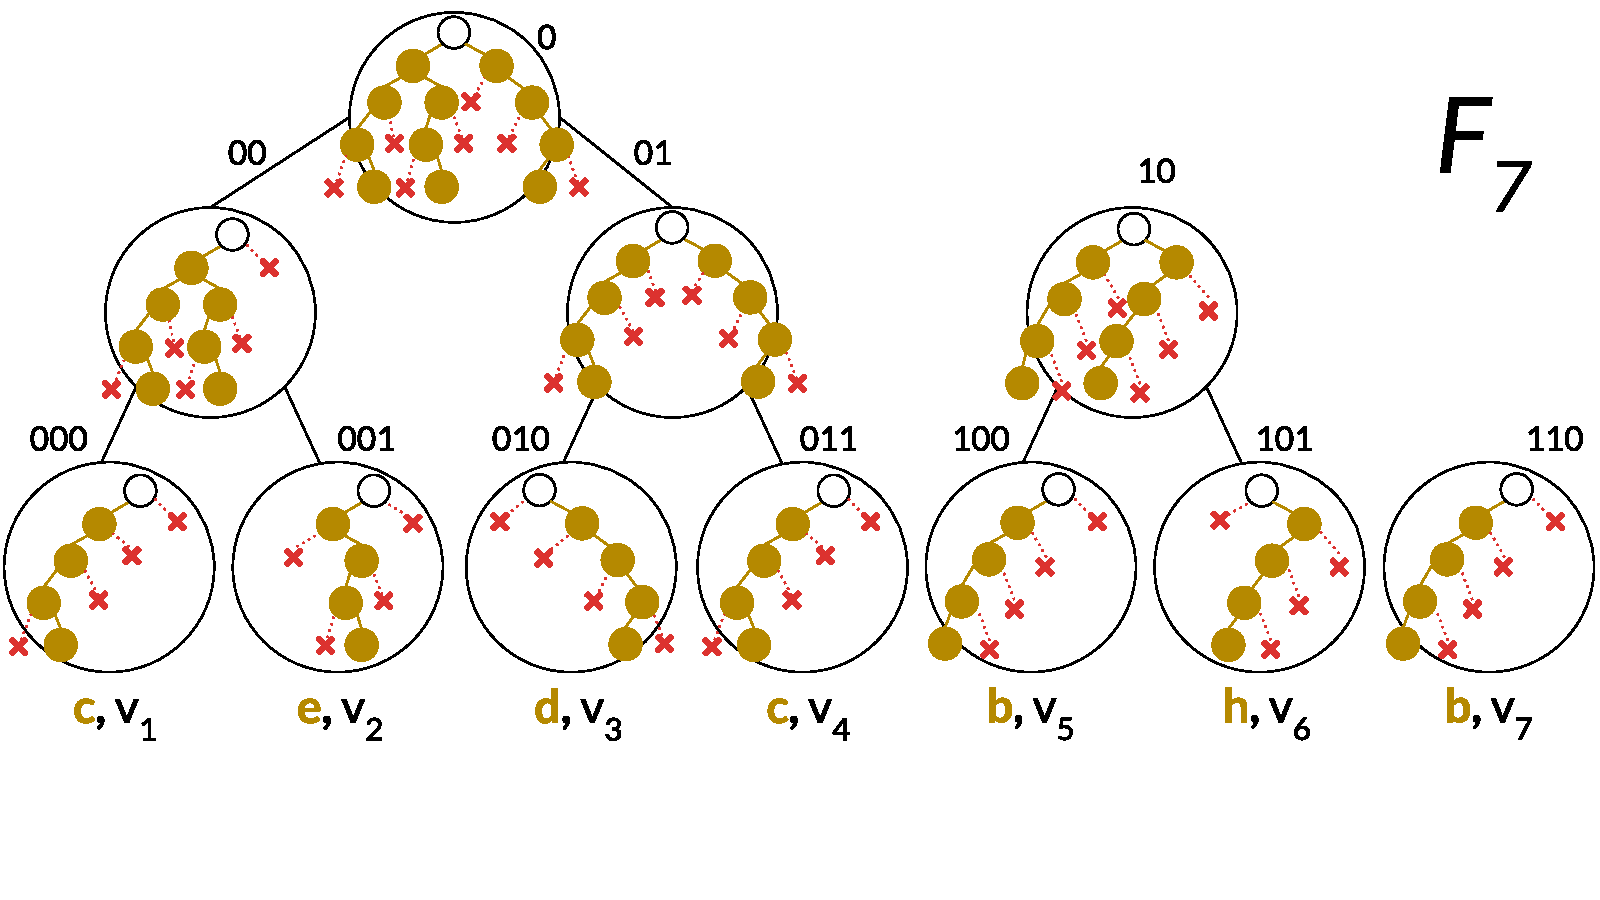
\includegraphics[width=.90\columnwidth]{figures-aad/accaad-short.pdf}
    \vspace{-1.7cm}
    \caption{
        A dynamic AAD for dictionary $\{(b,v_5),(b,v_7),(c,v_1),(c,v_4),(d,v_3),(e,v_2),(h,v_6)\}$ with $\lambda=2$.
        Unlike the AAS from \cref{f:accaas}, this AAD stores key-value pairs in the forest leaves.
        Furthermore, \textit{every node} in the forest now stores a \frontierCommunionTree (FCT).
        Similar to the AAS, all accumulators are built over the prefixes of the keys.
        This way, the accumulators can be used to ``provably-guide'' a search for all the values of a key.
    }
    \label{f:accaad-short}
\end{figure}

We can easily modify our AAS approach from \cref{s:aas:from-bilinear-acc} to obtain an AAD as depicted in \cref{f:accaad-short}.
First, the leaves in the forest will now store \textit{key-value pairs}, since we want dictionaries rather than sets.
As before, each node in the forest will store a prefix accumulator, but the accumulator will be computed only over the keys in its subtrees, even though the leaves store key-value pairs.
Thus, each tree in the forest can be regarded as a PCT, which stores key-value pairs as leaves but only accumulates the keys.
This will be very useful for proving lookups.

Second, all nodes in the forest, not just root nodes, need to store an FCT.
(In contrast, in our AAS, only root nodes stored FCTs, and internal nodes discarded them after merges.)
The FCTs enable the server to easily prove that a key $k$ is \textit{not} in a node's subtree.
This is necessary for proving lookups.
On the other hand, FCTs at every node increase the space on the server to $O(\lambda n \log{n})$.
Finally, append-only proofs remain the same as in the AAS.
We can now detail exactly how lookup proofs work.

\subsubsection{Proving Lookups}
\label{s:aad:from-acc:short:lookup-proofs}
Consider lookups for a key $k$ with a single value $v$.
Equipped with the ability of proving non-membership of $k$ in any node in the forest, the server can now easily prove such lookups.
First, the server shows $(k,v)$ is in a PCT using a proof path.
Second, to show that $k$ has no other values in that tree, the server proves $k$ is \textit{not} in any of the subtrees rooted at the sibling nodes along the proof path.
We call these subtrees \textit{missing subtrees}, since only their roots are included in the PCT proof path (as sibling nodes).
For every missing subtree, the server gives a frontier proof for $k$ not being there.
Finally, for all other PCTs in the forest, the server gives a frontier proof that $k$ is not in that PCT.

We can now generalize.
Suppose $k$ has (zero or more) values $V$ ``spread out'' across $t$ of the $O(\log{n})$ trees in the forest.
The lookup proof consists of:
\begin{itemize}
    \item For each value $v\in V$, a PCT proof path to $(k,v)$ in the forest. These paths add $O(|V|\log{n})$ overhead and form what we call a \textit{pruned forest}.
    \item For each missing subtree in this pruned forest, a frontier proof for $k$ in that subtree. There will be $O(|V|\log{n})$ such subtrees (and thus frontier proofs).
    \item For each of the $\log{(n)}-t$ remaining PCTs where $k$ has no values, a frontier proof to prove $k$ is not there. This is at most $O(\log{n})$ frontier proofs.
\end{itemize}
Thus, the lookup proof size is $O\left(|V|\log{n} + f(|V|\log{n} + \log{n})\right)$, where $f$ is the frontier proof size.
If instantiated with RSA accumulators, we call this scheme \rsaaadset, and it has $O(|V|\log{n})$ lookup proofs.
If instantiated with bilinear accumulators, we call it \biaadset, and it has $O(|V|\log^2{n})$ lookup proofs.

\subsection{AADs with Less Space Overhead}
\label{s:aad:from-acc:tall}
\begin{figure}[t]
    \centering
    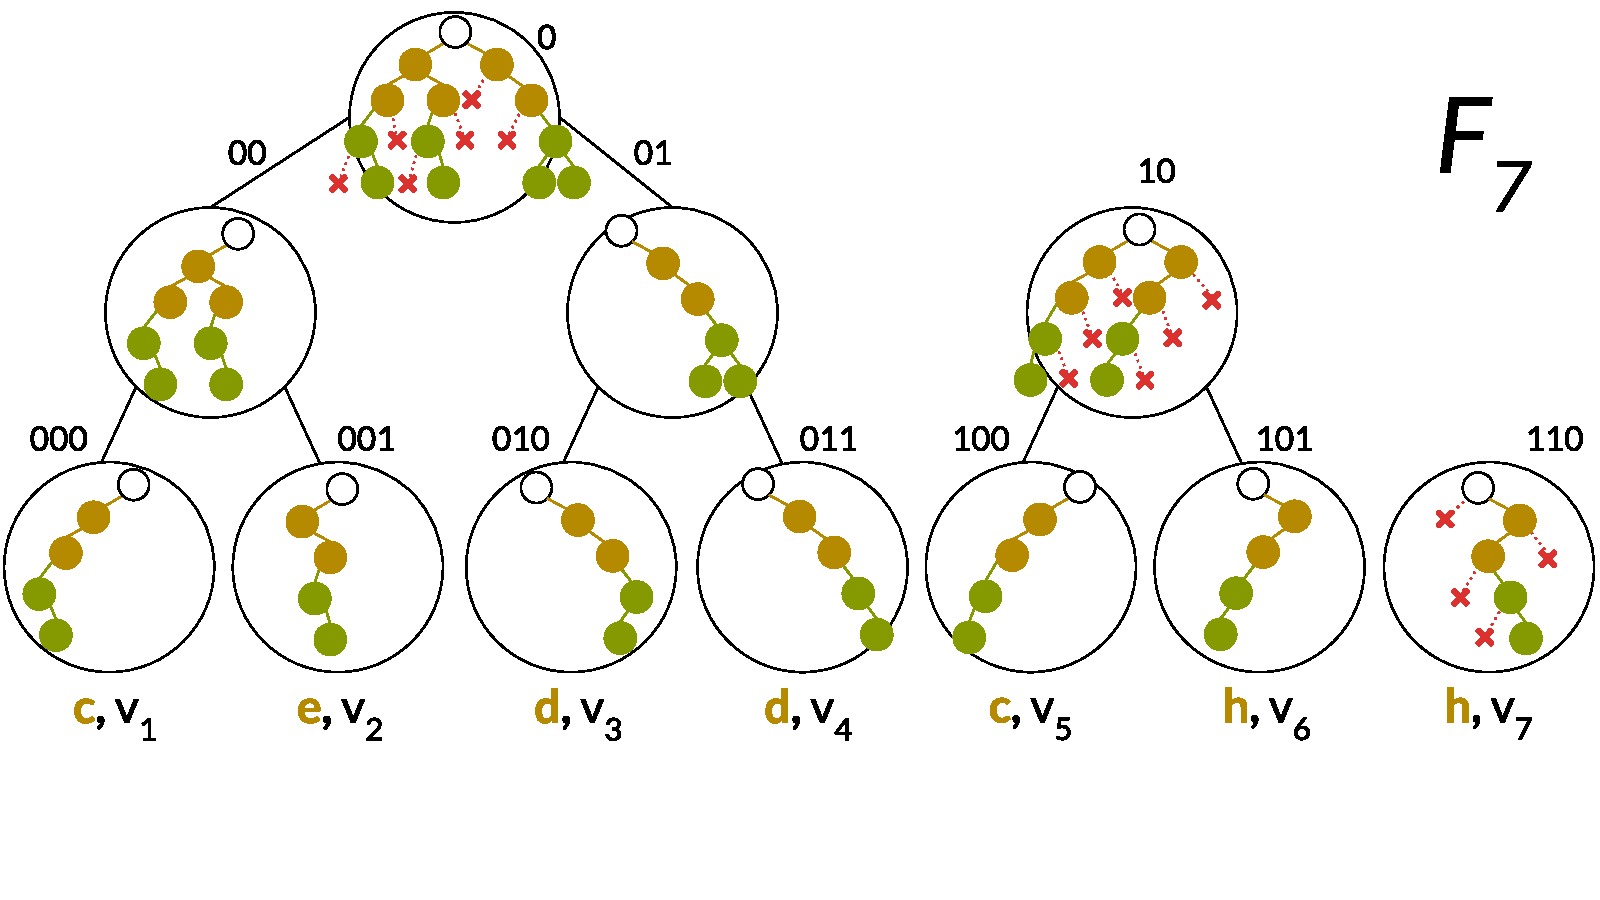
\includegraphics[width=.90\columnwidth]{figures-aad/accaad-tall.pdf}
    \vspace{-1.7cm}
    \caption{
        A dynamic AAD for dictionary $\{(c,v_1),(c,v_5),(d,v_3),(d,v_4),(e,v_2),(h,v_6),(h,v_7)\}$ with $\lambda=1$.
        The tries in this AAD are built not just over keys but also over values, unlike our AAS from \cref{f:accaas} and unlike our ``short'' AAD from \cref{f:accaad-short}.
        Specifically, the first $2\lambda$ edges in a trie path encode the hash of the key and the last $2\lambda$ edges encode the hash of the value.
        As in our AAS, \textit{only root nodes} in the forest store a \frontierCommunionTree (FCT).
        These root FCTs are used to ``provably-guide'' a search for all the values of a key.
    }
    \label{f:accaad-tall}
\end{figure}

Here, we take a different approach where PCTs accumulate both keys and their values in a manner that allows us to construct lookup proofs.
Specifically, we increase the size of the domain of the underlying AAS from $2\lambda$ bits to $4\lambda$ bits so as to account for the value $v$, as depicted in \cref{f:accaad-tall}.
That is, $(k,v)$ would be inserted in the AAS as $k|v$, using the same algorithms from \cref{s:aas:from-bilinear-acc:algorithms}.
This increases the trie height, making appends slower since more prefixes have to be accumulated.
We call the RSA-based construction \rsaaad and the bilinear-based construction \biaad.

Note that \biaad has double the $q$-PKE parameters public parameters of \biaas (and of \biaadset).
Specifically, the server needs $q=4\lambda n + 1$ and clients need $q=4\lambda+1$.
% More precisely, clients only need (g^{\tau^i})_{i\in[0,4\lambda+1]} since they never need to reconstruct extractable accumulators
On the other hand, \biaad and \rsaaad have lower space overhead than \biaadset and \rsaaad: $O(\lambda n)$ versus $O(\lambda n\log{n})$.

\paragraph{Supporting Large Domains and Multisets.}
To handle keys and values longer than $2\lambda$ bits, we store $\mathcal{H}(k)|\mathcal{H}(v)$ in the AAD (rather than $k|v$), where $\mathcal{H}$ is a CRHF and we can retrieve the actual value $v$ from another repository.
To support multisets (same $v$ can be inserted twice for a $k$), the server can insert $\mathcal{H}(\mathcal{H}(v)|i)$ for the $i$th occurrence of $(k,v)$.
% Simply inserting H(k)|H(v) does not work because if you insert (k,v) twice, and both insertions end up in the same PCT, then the frontier cannot be used to guarantee all copies of the same value $v$ have been revealed by the prover.
% In fact, the frontier is not even used here: the prover just gives a path to one of the (k,v)'s and then uses the frontier to show that there are not other values other than v for k in this PCT.
% The problem is that while that might be true, it does not say anything about how many times the value v occurrs in the PCT.

\subsubsection{Proving Lookups}
\label{s:aad:from-acc:tall:lookup-proofs}

First, consider a key $k$ with no values.
A lookup proof consists of $O(\log{n})$ frontier proofs, one for each PCT in the forest where a prefix of $k$ is missing.
This is very similar to a non-membership proof in the AAS (see \cref{s:aas:from-bilinear-acc}).

But what if $k$ has one or more values?
First, the lookup proof contains paths to PCT leaves with $k$'s values (i.e., with elements of the form $k|v$), much like a membership proof in an AAS.
But what is to guarantee \textit{completeness} of the response?
What if a malicious server leaves out one of the values of key $k$?
(This is important in transparency logs where users look up their own PKs and must receive all of them to detect impersonation attacks.)

\paragraph{Lower Frontiers.}
\begin{figure}[t]
    \centering
    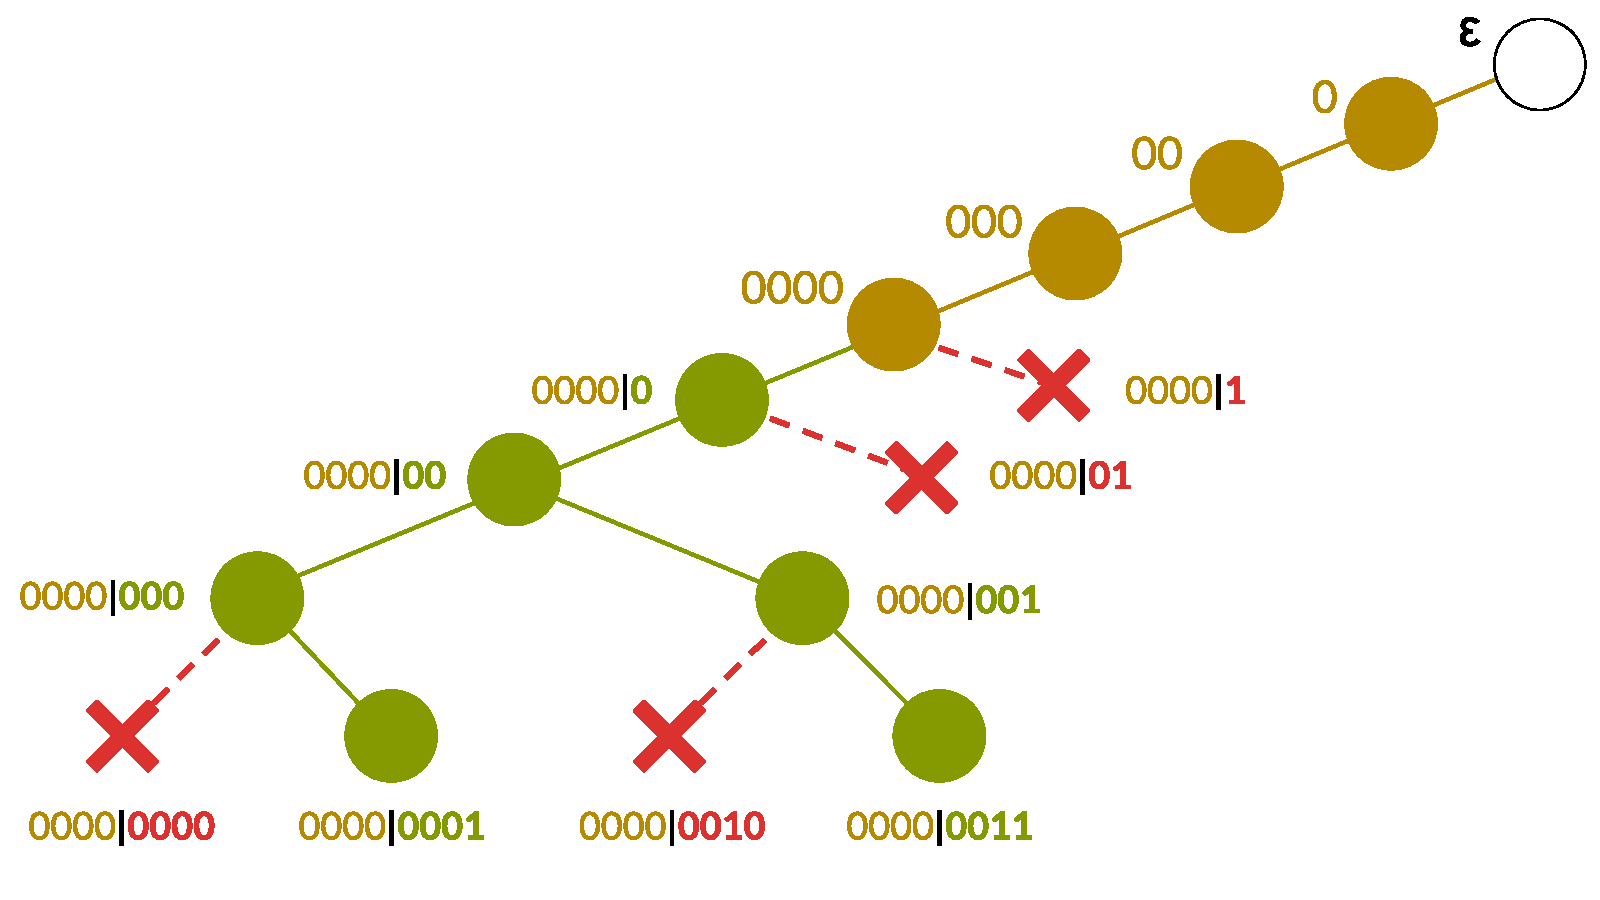
\includegraphics[width=\columnwidth]{figures-aad/lower-frontier.pdf}
    \vspace{-1.0cm}
    \caption{
        A ``tall'' trie for a key $k$ with hash $0000$ that has two values with hashes $0001$ and $0011$, respectively.
        The security parameter is $\lambda=2$.
        The lower frontier consists of the \red{red nodes} in the lower half of the trie, which correspond to missing values for $k$.
    }
    \label{f:lower-frontier}
\end{figure}
We use the same frontier technique as in the AAS to convince clients values are not being left out.
Specifically, the server proves specific prefixes for the \textit{missing values} of $k$ are not in the PCTs (and thus are not maliciously being left out).
This is best illustrated with the example in \cref{f:lower-frontier} where the security parameter is $\lambda=2$.

Suppose the server wants to prove $k=0000$ has \textit{complete} set of values $V=\{v_1 = 0001, v_2 = 0011\}$.
Consider a trie over $k|v_1$ and $k|v_2$ and note that $F^{[k]}_V = \{(0000|1), (0000|01), (0000|0000)$, $(0000|0010)\}$ is the set of all frontier prefixes for the missing values of $k$.
We call this set the \textit{lower frontier} of $k$ relative to $V$.
The key idea for showing completeness of $V$ is to \textit{prove all these lower frontier prefixes are in the FCT} via frontier proofs (as defined in \cref{s:aas:from-bilinear-acc}).
Since there are $O(\lambda)$ lower frontier prefixes, one for each value $v\in V$ of key $k$, the server will send $O(\lambda|V|)$ frontier proofs.
Thus, a proof for a key $k$ with a single value $v$ (i.e., $V=\{v\}$) consists of:
\begin{itemize}
    \item A proof path to $(k,v)$ in some PCT (to show $v$ is one of $k$'s values),
    \item $O(\lambda)$ frontier proofs in the FCT corresponding to that PCT, one for each prefix in the lower frontier $F^{[k]}_{\{v\}}$ (to guarantee completeness of $\{v\}$ in that PCT),
    \item A frontier proof for a missing prefix of $k$ in each one of the remaining $O(\log{n})$ FCTs (to prove $k$ has no values there).
\end{itemize}

\paragraph{Keys with Multiple Values.}
Let us generalize lookup proofs to keys with many values.
Assume the key $k$ has (zero or more) values in $V$ that are ``spread out'' across $t\ge 0$ of the $\le \log{n}$ PCTs in the forest.
For PCTs with no values for $k$, the server proves non-membership of $k$ in the corresponding FCT via one frontier proof.
For the $i$th PCT, where $k$ has values $v \in V_i$, the server proves the completeness of $V_i$ by giving $O(\lambda|V_i|)$ frontier proofs, one for each lower frontier prefix.
Thus, the lookup proof consists of:

\begin{itemize}
    \item For each value $v\in V$, a PCT proof path to $(k,v)$ in the forest. These add $O(|V|\log{n})$ overhead.
    \item Across the $t$ PCTs where $k$ has values, $O(\lambda|V|)$ frontier proofs will be sent.
    \item For each of the $\log{(n)}-t$ remaining PCTs where $k$ has no values, a frontier proof in its corresponding FCT to prove $k$ is not there.
\end{itemize}

Thus, the total number of frontier proofs is $O\left(\lambda|V| - t + \log{n}\right)=O\left(\lambda|V| + \log{n}\right)$.
This means the lookup proof size is $O\left(f\left(\lambda|V| + \log{n}\right) + |V|\log{n}\right)$-sized, where $f$ is the construction-specific frontier proof size.
%Now let us consider the general case of a key with values $V=\bigcup_{i\in[\log{n}]} V_i$, where $V_i$ are the values of $k$ in the $i$th tree in the forest (if any) and $t$ is the number of trees for which $V_i\ne \varnothing$.
%$O\left(\left(\sum_{i=1}^t {\lambda|V_i|}\right) - t + \log{n})\right)$ where $0 \le t\le \log{n}$.
% Because, for every tree where k has a value, the complexity goes from (\lambda + \log{n}) frontier proofs, to (\lambda + \lambda + (\log{n} - 1)) frontier proofs.
%
% All values V could be in a single tree: $O(\lambda|V|)$ frontier proofs in that tree + $O(\log{n})$ frontier proofs, one for the remaining trees
% All values V could be spread out in all trees: $O(\lambda|V|)$ frontier proofs across all tree
% Somewhere in between: $O(\lambda|V|)$ across \log{n}/2 trees + \log{n}/2 frontier proofs, one for each remaining tree
Next, we describe how to remove the $\lambda$ factor in the expression above.
% and decrease it to $O\left(f\left(|V| + \log{n}\right) + |V|\log{n}\right)$,
 
\paragraph{Smaller Lookup Proofs in \biaad.}
Since frontier proofs are $O(\log{n})$-sized, the \biaad lookup proof size will be $O(\lambda |V|\log{n}+\log^2{n})$.
% b.c., just apply $f=O(\log{n})$ in the expression from the paragraph above.
% e.g., when there are values in all trees.
% e.g., when there aren't, you have to add another \log^2{n} factor which is dominated away by \lambda\log{n}.
We show how to decrease this to $O(|V|\log{n} + \log^2{n})$.
% All values V could be in a single tree: $O(|V|\log{n})$ for that tree + $O(\log^2{n})$ for the remaining trees
% All values V could be spread out in all trees: $O(|V|\log{n})$ frontier proofs across all tree
% Somewhere in between: $O(\lambda|V|)$ across \log{n}/2 trees + \log{n}/2 frontier proofs, one for each remaining tree
We begin with the case where $k$ has one value.

We know from before that a lookup proof for $(k,\{v\})$ is $O(\lambda \log{n})$-sized
(since the $\lambda\log{n}$ term dominates the $\log^2{n}$ term).
Note that the $O(\lambda)$ overhead comes from having to prove that all $O(\lambda)$ \underline{lower} frontier prefixes of $k$ (relative to $V$) are in an FCT.
The key idea is to \textit{group all these lower frontier prefixes} into a single FCT leaf, creating a frontier accumulator over all of them.
As a result, instead of having to send $O(\lambda)$ frontier proofs (one for each lower frontier prefix), we send a single $O(\log{n})$-sized frontier proof for a single FCT leaf which contains all $O(\lambda)$ lower frontier prefixes of $k$ relative to $\{v\}$.

We can generalize this idea. 
Specifically, if $k$ has $|V_i|$ values in the $i$th FCT in the forest, then $k$'s lower frontier relative to $V_i$ has $O(\lambda|V_i|)$ prefixes.
Then, for each FCT $i$, we split the lower frontier prefixes of $k$ associated with $V_i$ into separate FCT leaves each of size at most $4\lambda + 1$.
We remind the reader that clients have enough public parameters to reconstruct the accumulators in these FCT leaves and verify the frontier proof.
% i.e., they have (g^{\tau^i})_{i=0}^{4\lambda+1}
As a result, the lookup proof size becomes $O(|V|\log{n} + \log^2{n})$.

\aadComplexityTable

\paragraph{Smaller Lookup Proofs in \rsaaad.}
Because frontier proofs are constant-sized in \rsaaas, the \rsaaad lookup proof size will be $O(\lambda |V|+\log{n}+|V|\log{n})$.
The same key idea from above can be used to bring the proof size down to $O(|V|+\log{n} + |V|\log{n})=O(|V|\log{n})$.
Recall that, in \rsaaad, constant-sized membership witnesses are computed for every frontier prefix.
Thus, in each FCT, for each key $k$'s lower frontier prefixes, we can aggregate its membership witnesses in batches of size $4\lambda+1$ using the technique from~\cite{BBF19}.

\subsection{Supporting Inclusion Proofs}
Another useful proof for a transparency log is an \textit{inclusion proof} which only returns \textit{one of the values} of key $k$ (while lookup proofs return \textit{all} values of a key $k$).
For example, in Certificate Transparency (CT), browsers are supposed to verify an inclusion proof of a website's certificate before using it.
Our AADs support inclusion proofs too.
They consist of a path to a PCT leaf with the desired key-value pair.
Since they do not require frontier proofs, inclusion proofs are only $O(\log{n})$-sized.

\subsection{Asymptotic Analysis}
\label{s:aad:from-acc:asymptotics}
We have already analyzed the lookup proof sizes of each construction in \cref{s:aad:from-acc:short:lookup-proofs,s:aad:from-acc:tall:lookup-proofs}.
The complexity analyses for the bilinear- and RSA-based AADs are similar to the ones from \cref{s:aas:from-bilinear-acc:asymptotics} and \cref{s:aas:from-rsa-acc:asymptotics}, respectively.
To avoid repetition, we give the AAD complexities in \cref{t:aad-from-acc-asymptotics}.